\begin{appendices}

\pagebreak

\chapter{Expanded Views of the Hardware Layout} \label{sec:appendix:expanded_layout}
Boards are 3" by 3"

\begin{figure}[ptb]
	\begin{centering}
		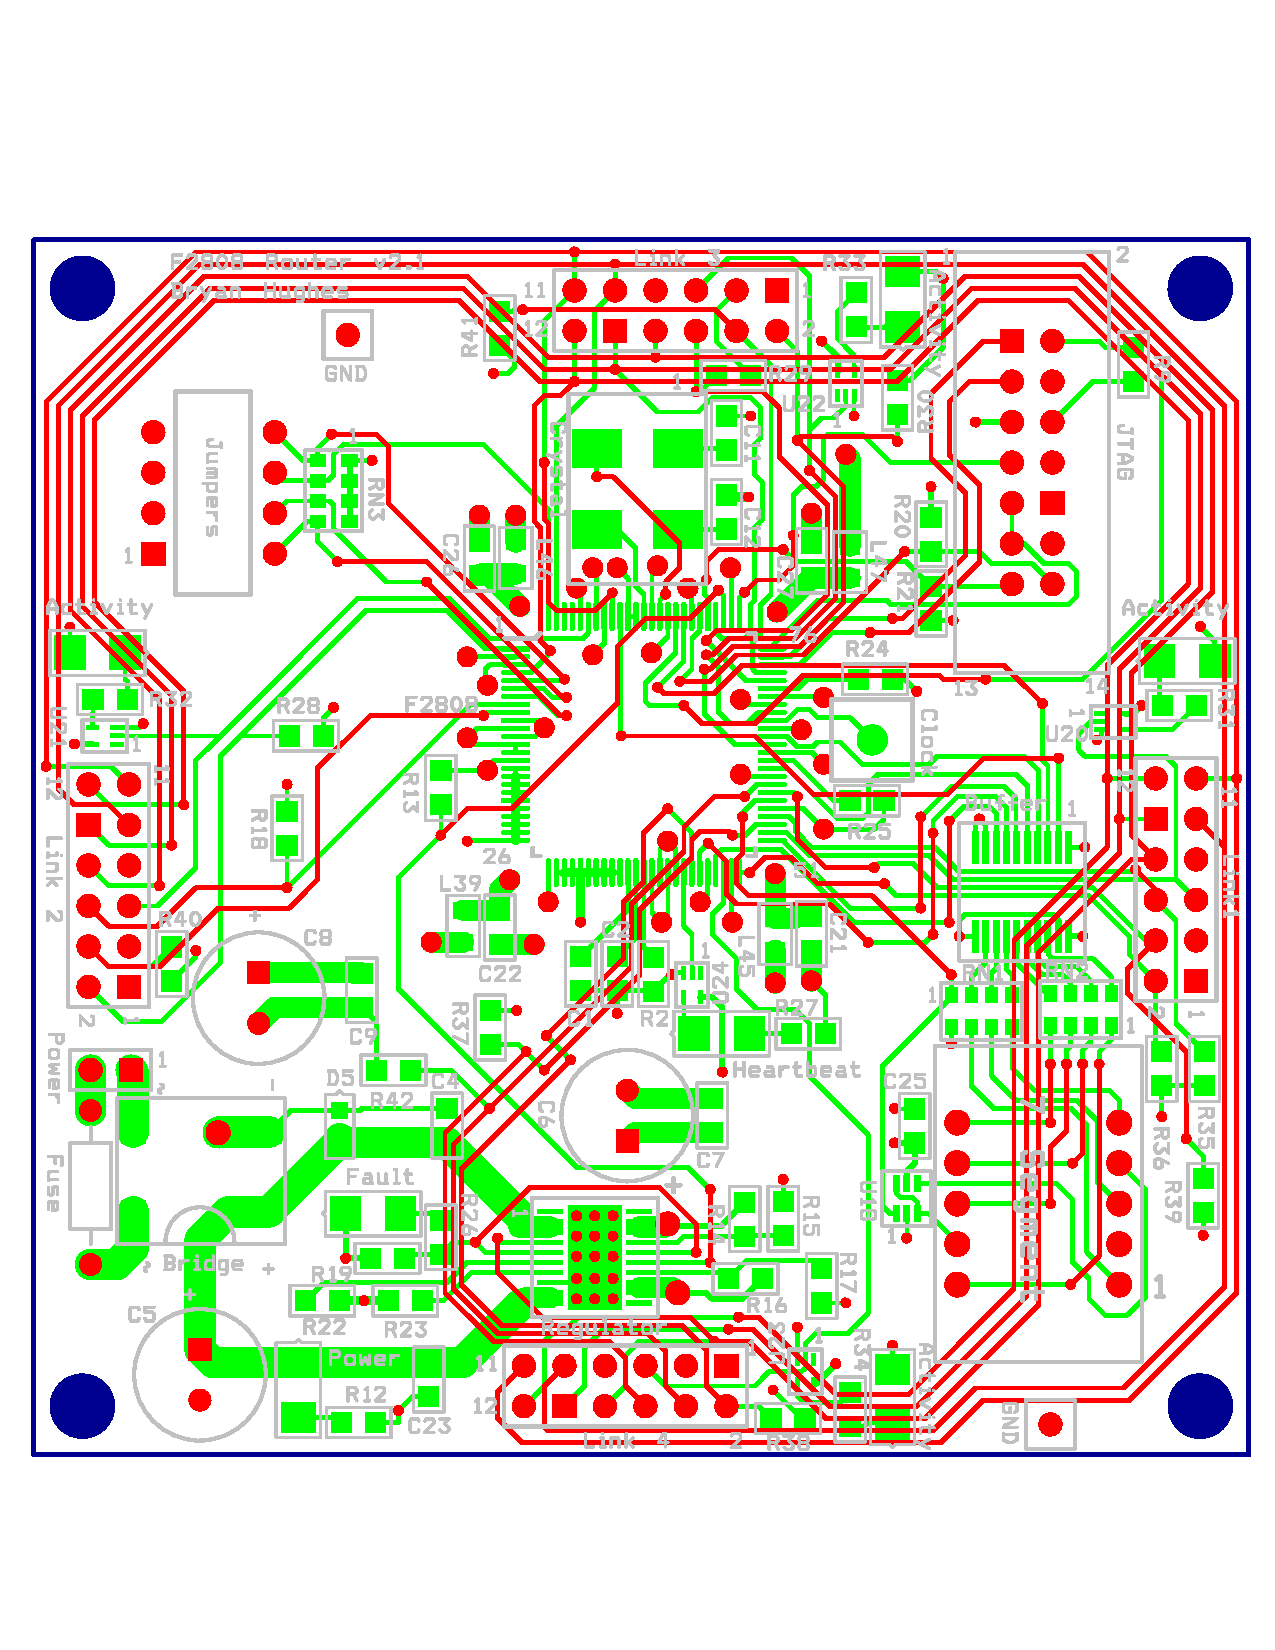
\includegraphics[width=6in]{Appendices/Figures/appendices-layout_no_power.pdf}
		\caption{Non-plane layers}
		\label{fig:appendices:layout_no_power}
	\end{centering}
\end{figure}

\begin{figure}[ptb]
	\begin{centering}
		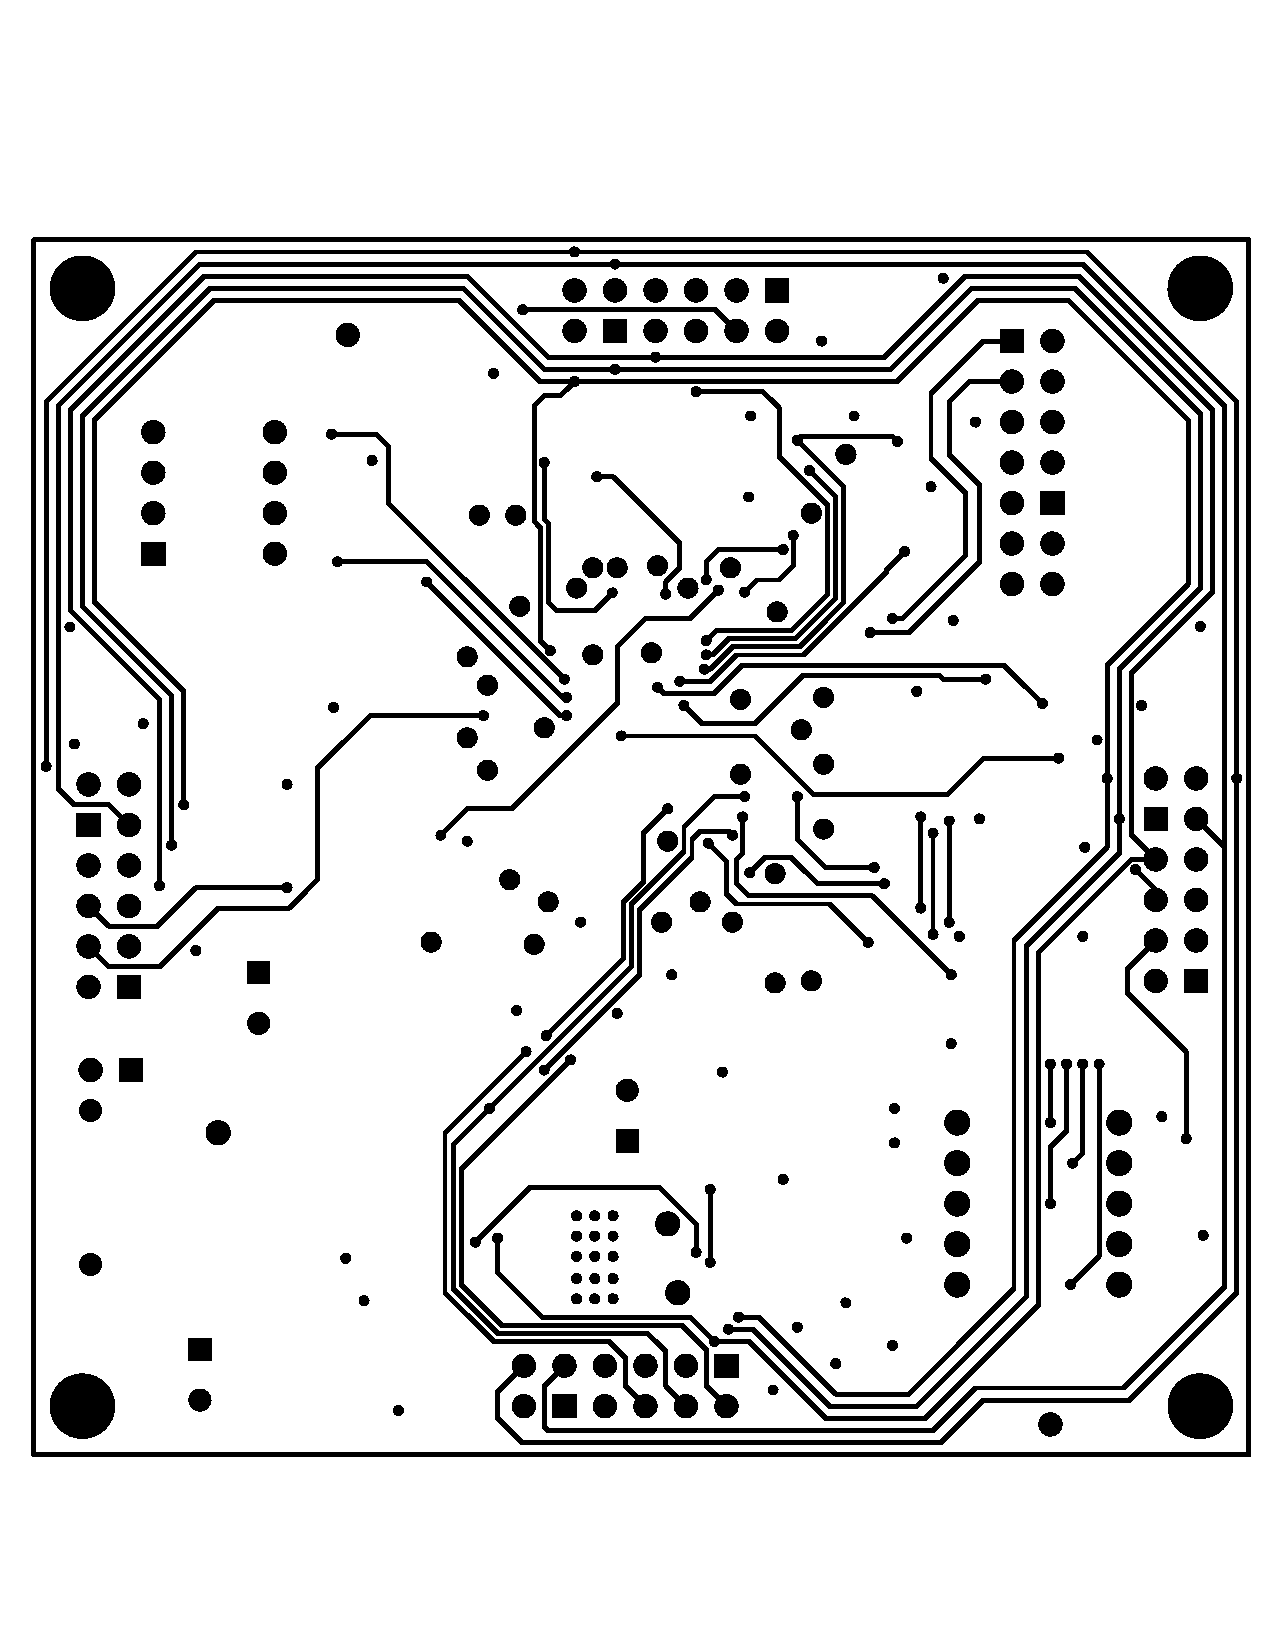
\includegraphics[width=6in]{Appendices/Figures/appendices-layout_bottom.pdf}
		\caption{Bottom layer}
		\label{fig:appendices:layout_bottom}
	\end{centering}
\end{figure}

\begin{figure}[ptb]
	\begin{centering}
		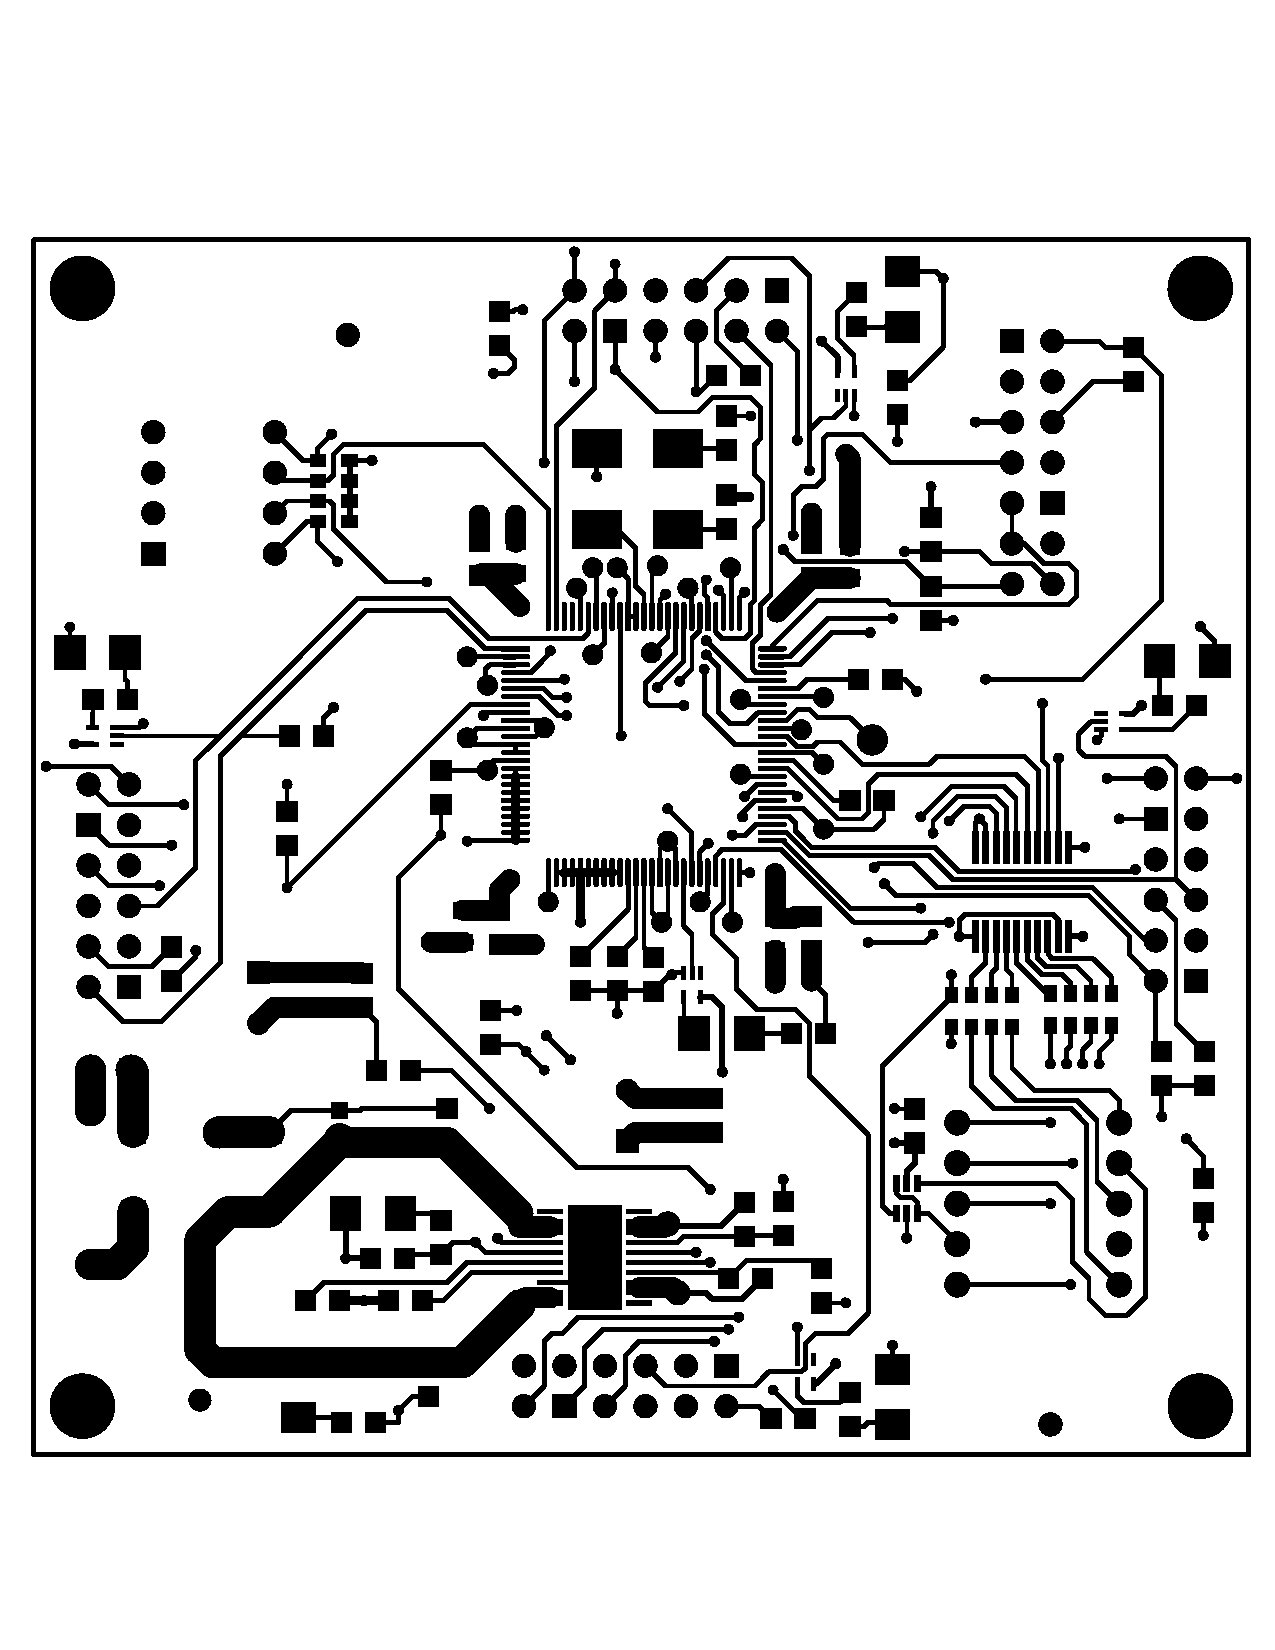
\includegraphics[width=6in]{Appendices/Figures/appendices-layout_top.pdf}
		\caption{Top layer}
		\label{fig:appendices:layout_top}
	\end{centering}
\end{figure}

\begin{figure}[ptb]
	\begin{centering}
		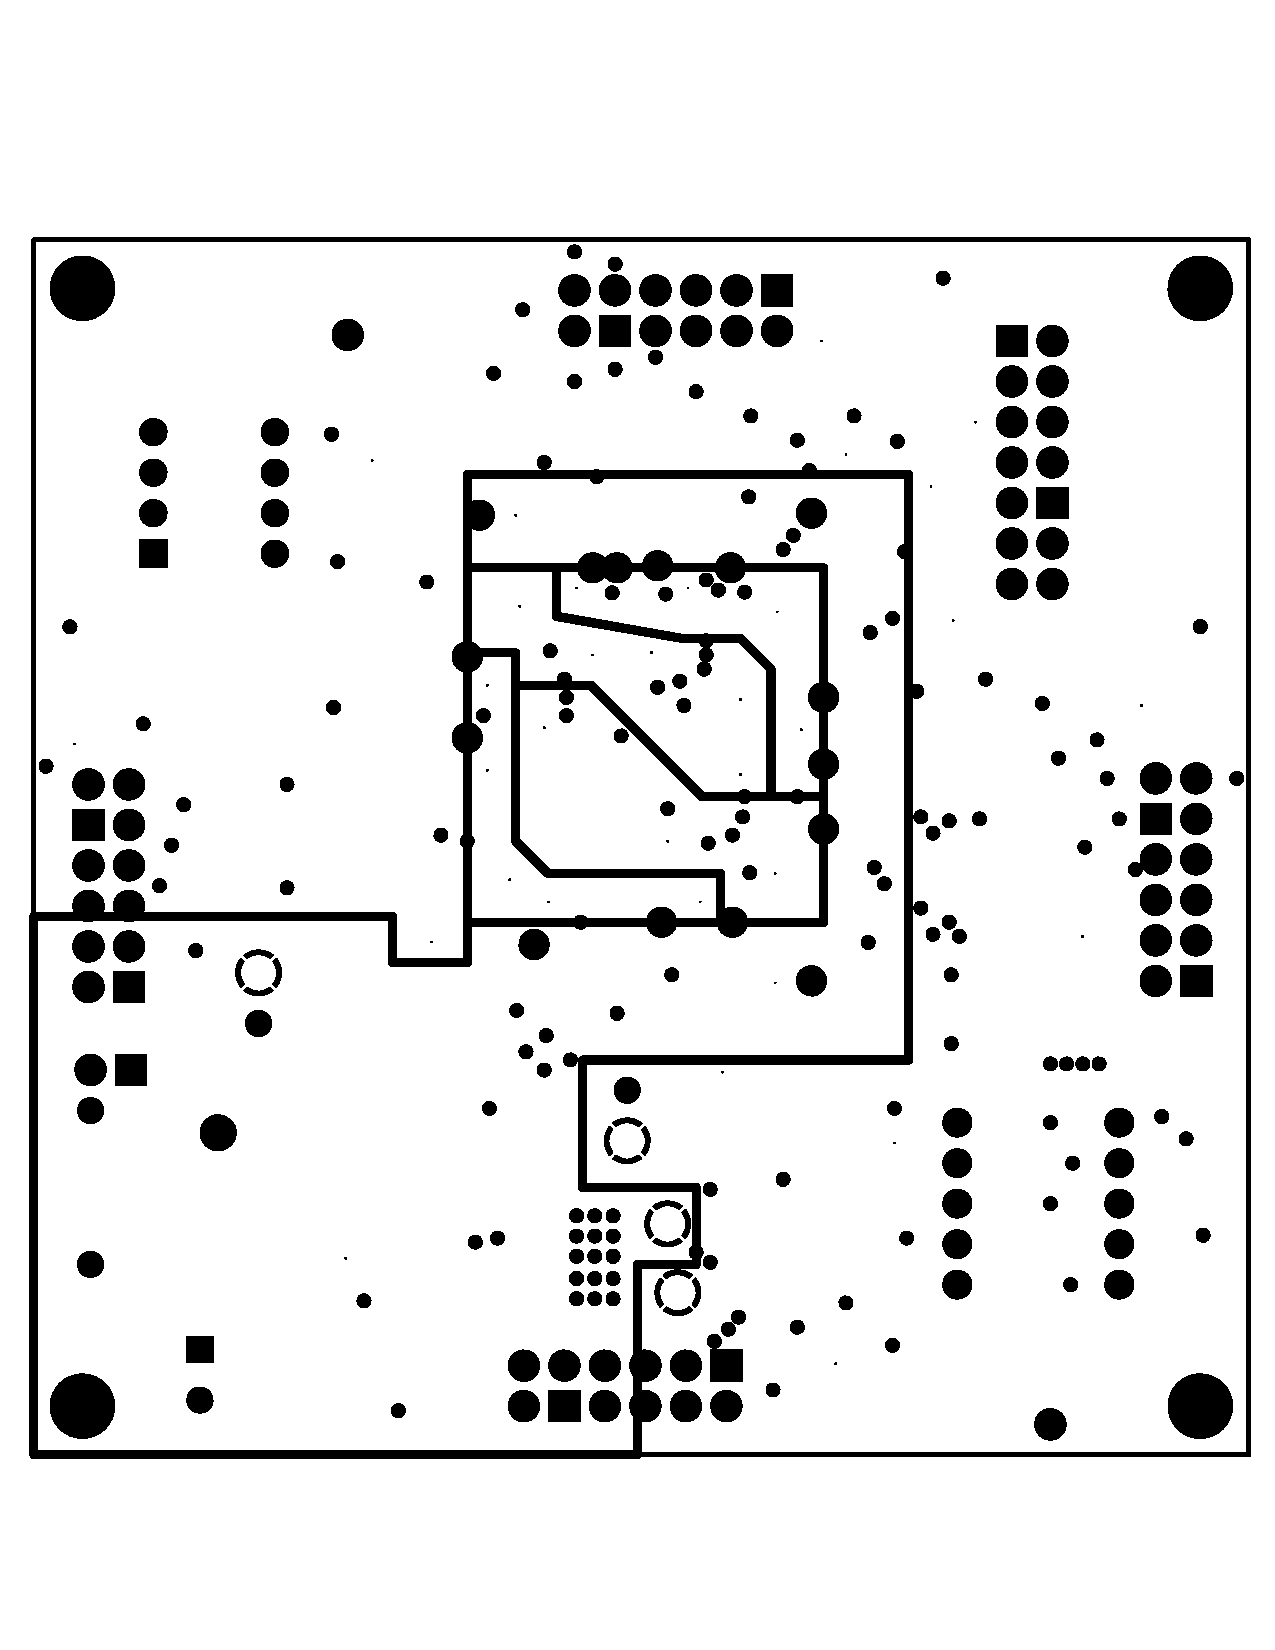
\includegraphics[width=6in]{Appendices/Figures/appendices-layout_power.pdf}
		\caption{Power plane}
		\label{fig:appendices:layout_power}
	\end{centering}
\end{figure}

\begin{figure}[ptb]
	\begin{centering}
		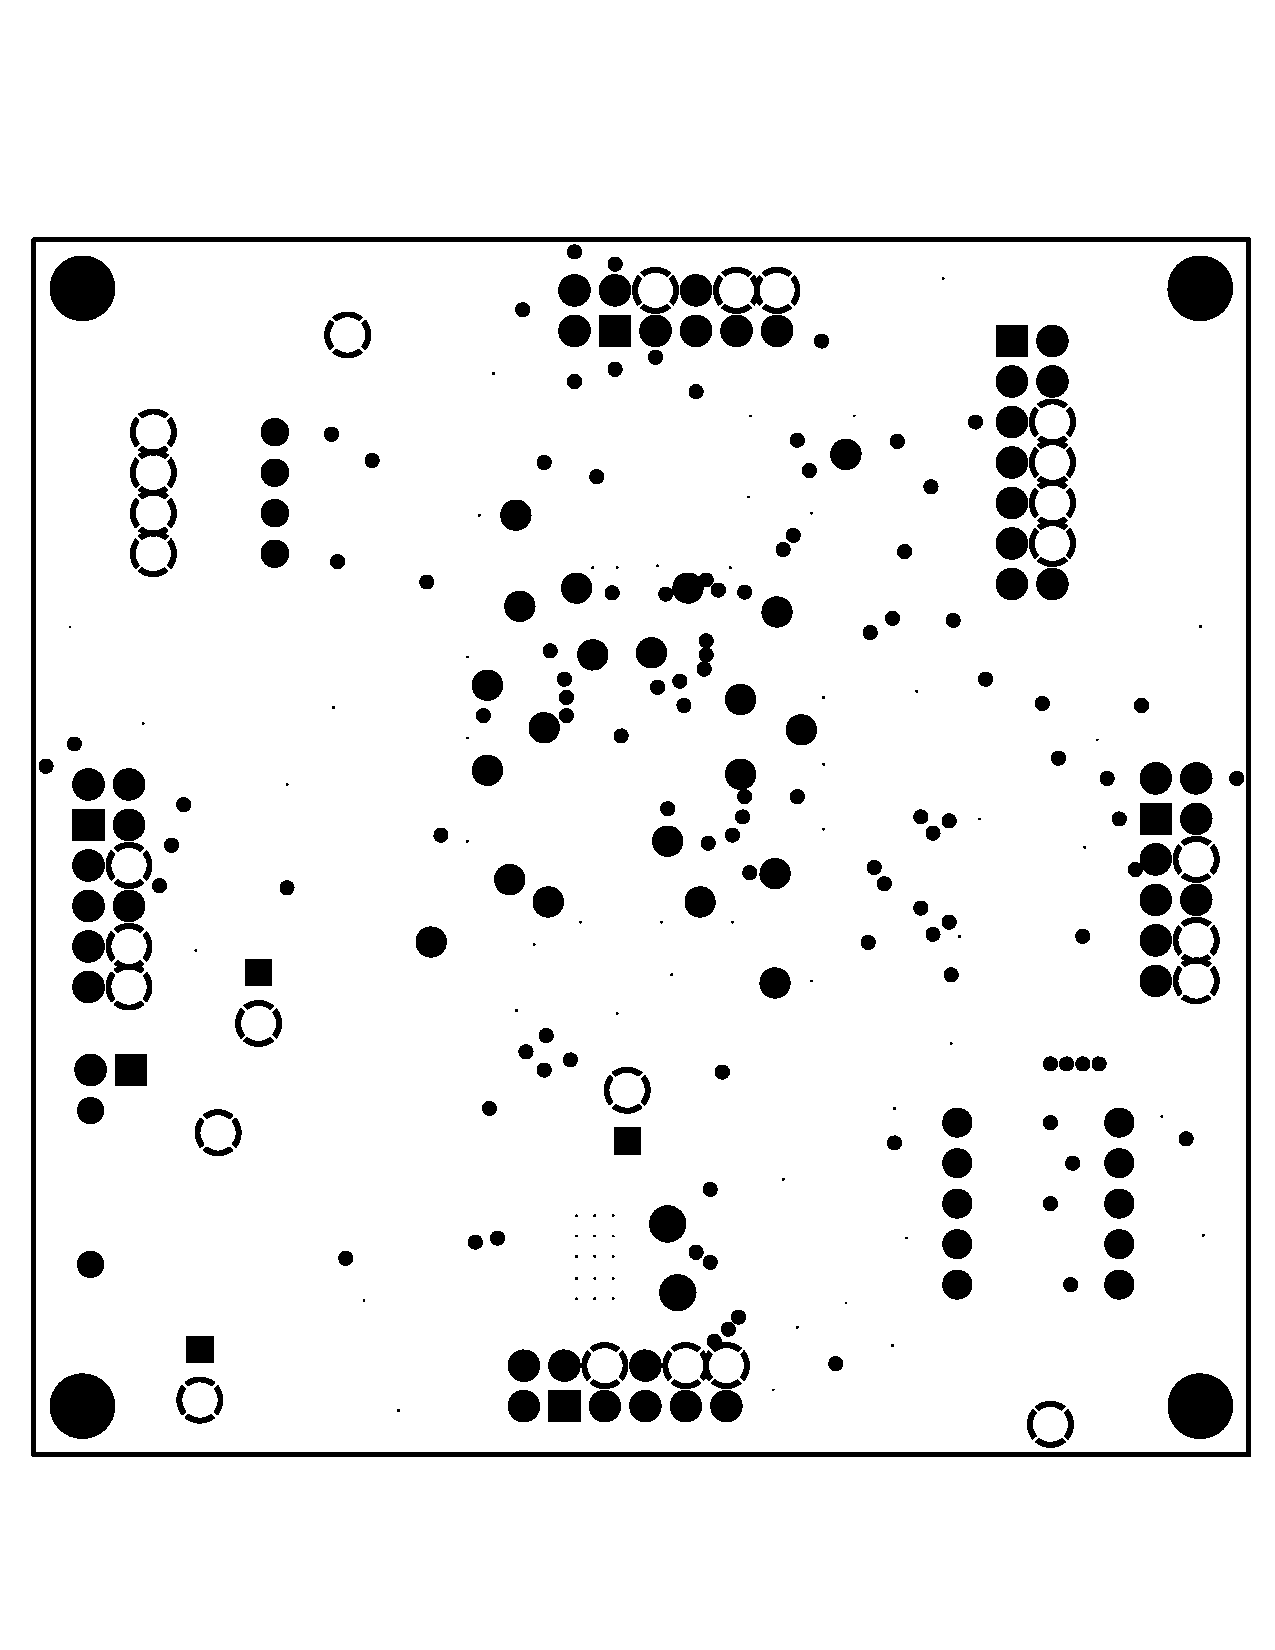
\includegraphics[width=6in]{Appendices/Figures/appendices-layout_ground.pdf}
		\caption{Ground plane}
		\label{fig:appendices:layout_ground}
	\end{centering}
\end{figure}

\begin{figure}[ptb]
	\begin{centering}
		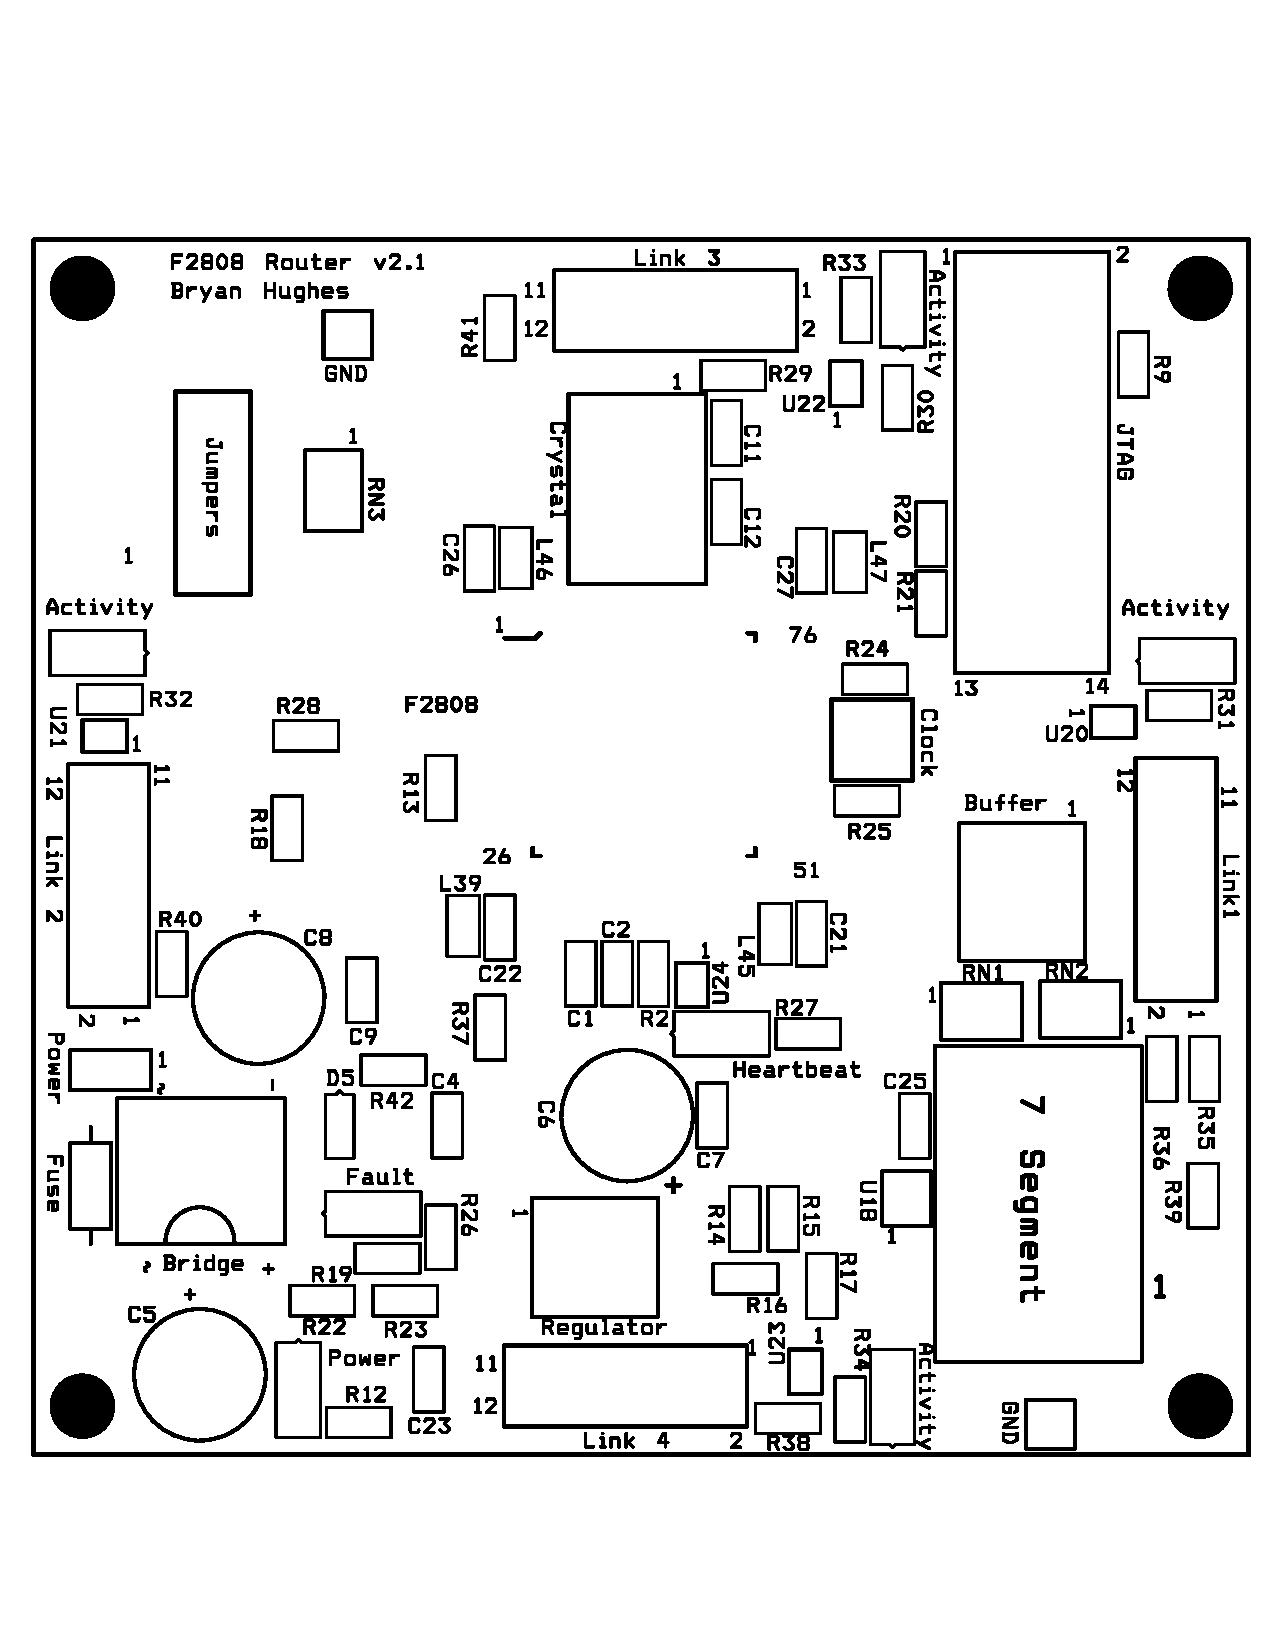
\includegraphics[width=6in]{Appendices/Figures/appendices-layout_silkscreen.pdf}
		\caption{Silkscreen layer}
		\label{fig:appendices:layout_silkscreen}
	\end{centering}
\end{figure}

\begin{figure}[ptb]
	\begin{centering}
		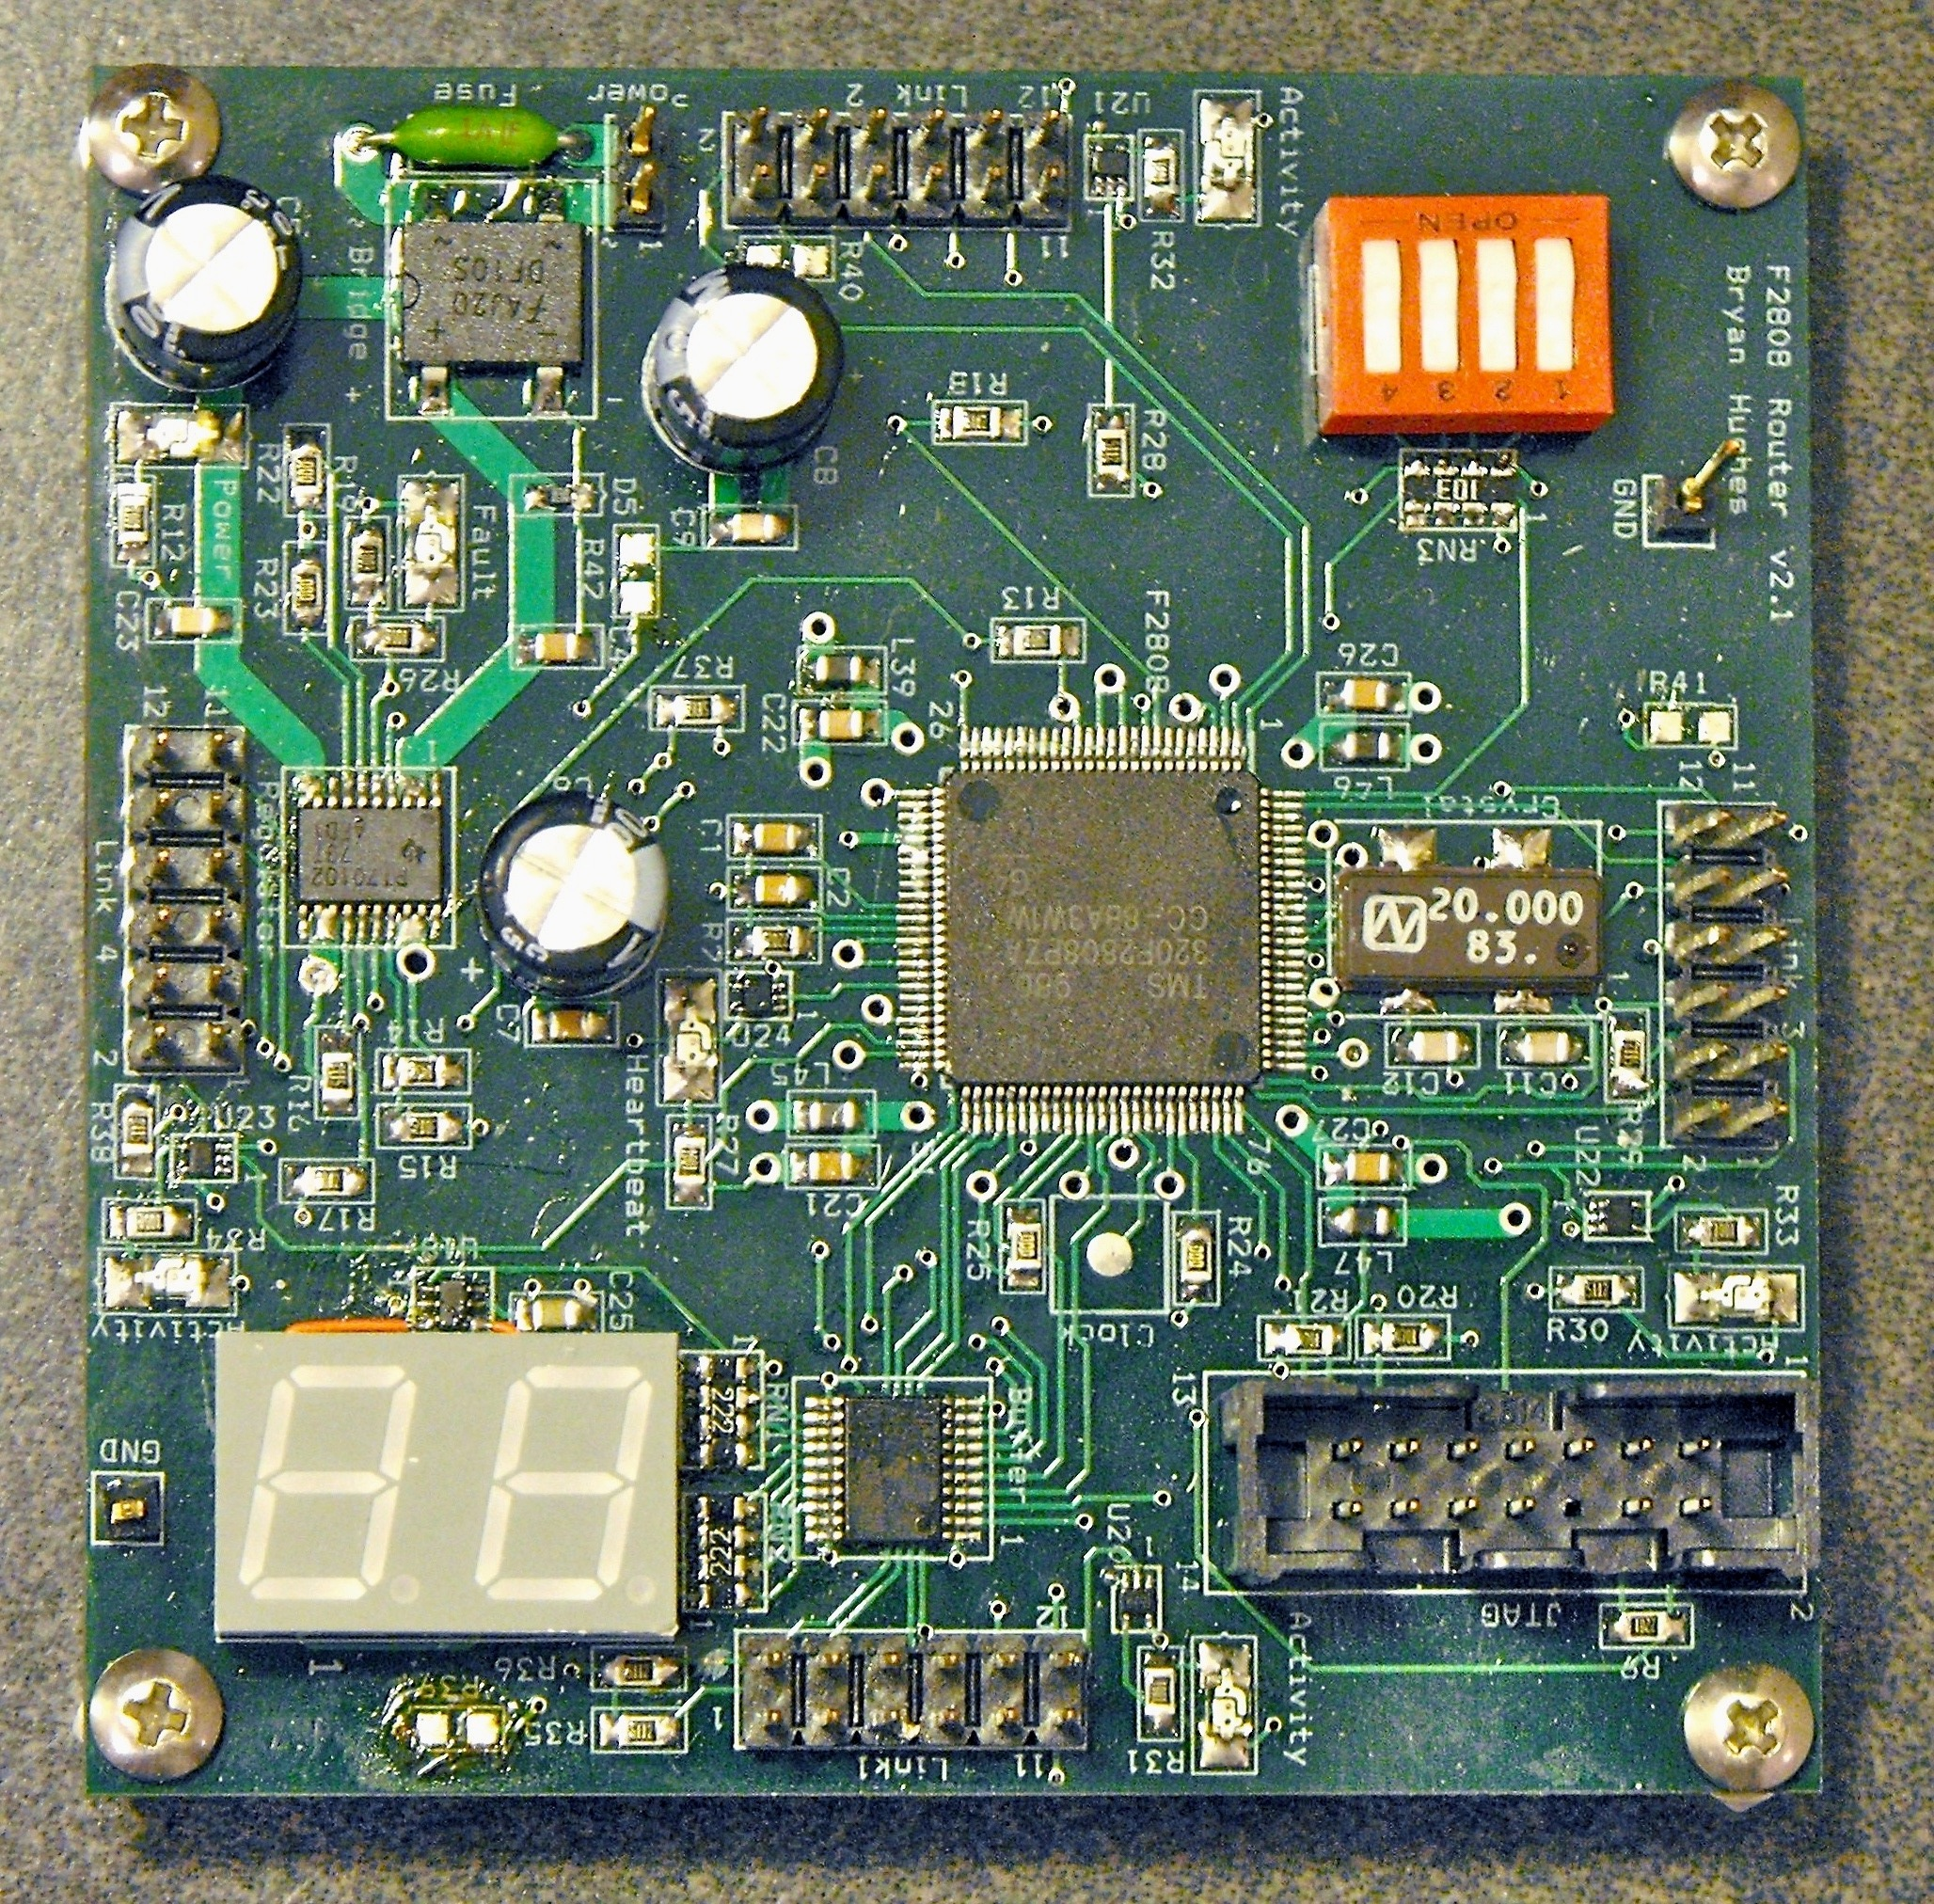
\includegraphics[width=6in]{Appendices/Figures/appendices-board_top.JPG}
		\caption{Top of the board}
		\label{fig:appendices:board_top}
	\end{centering}
\end{figure}

\begin{figure}[ptb]
	\begin{centering}
		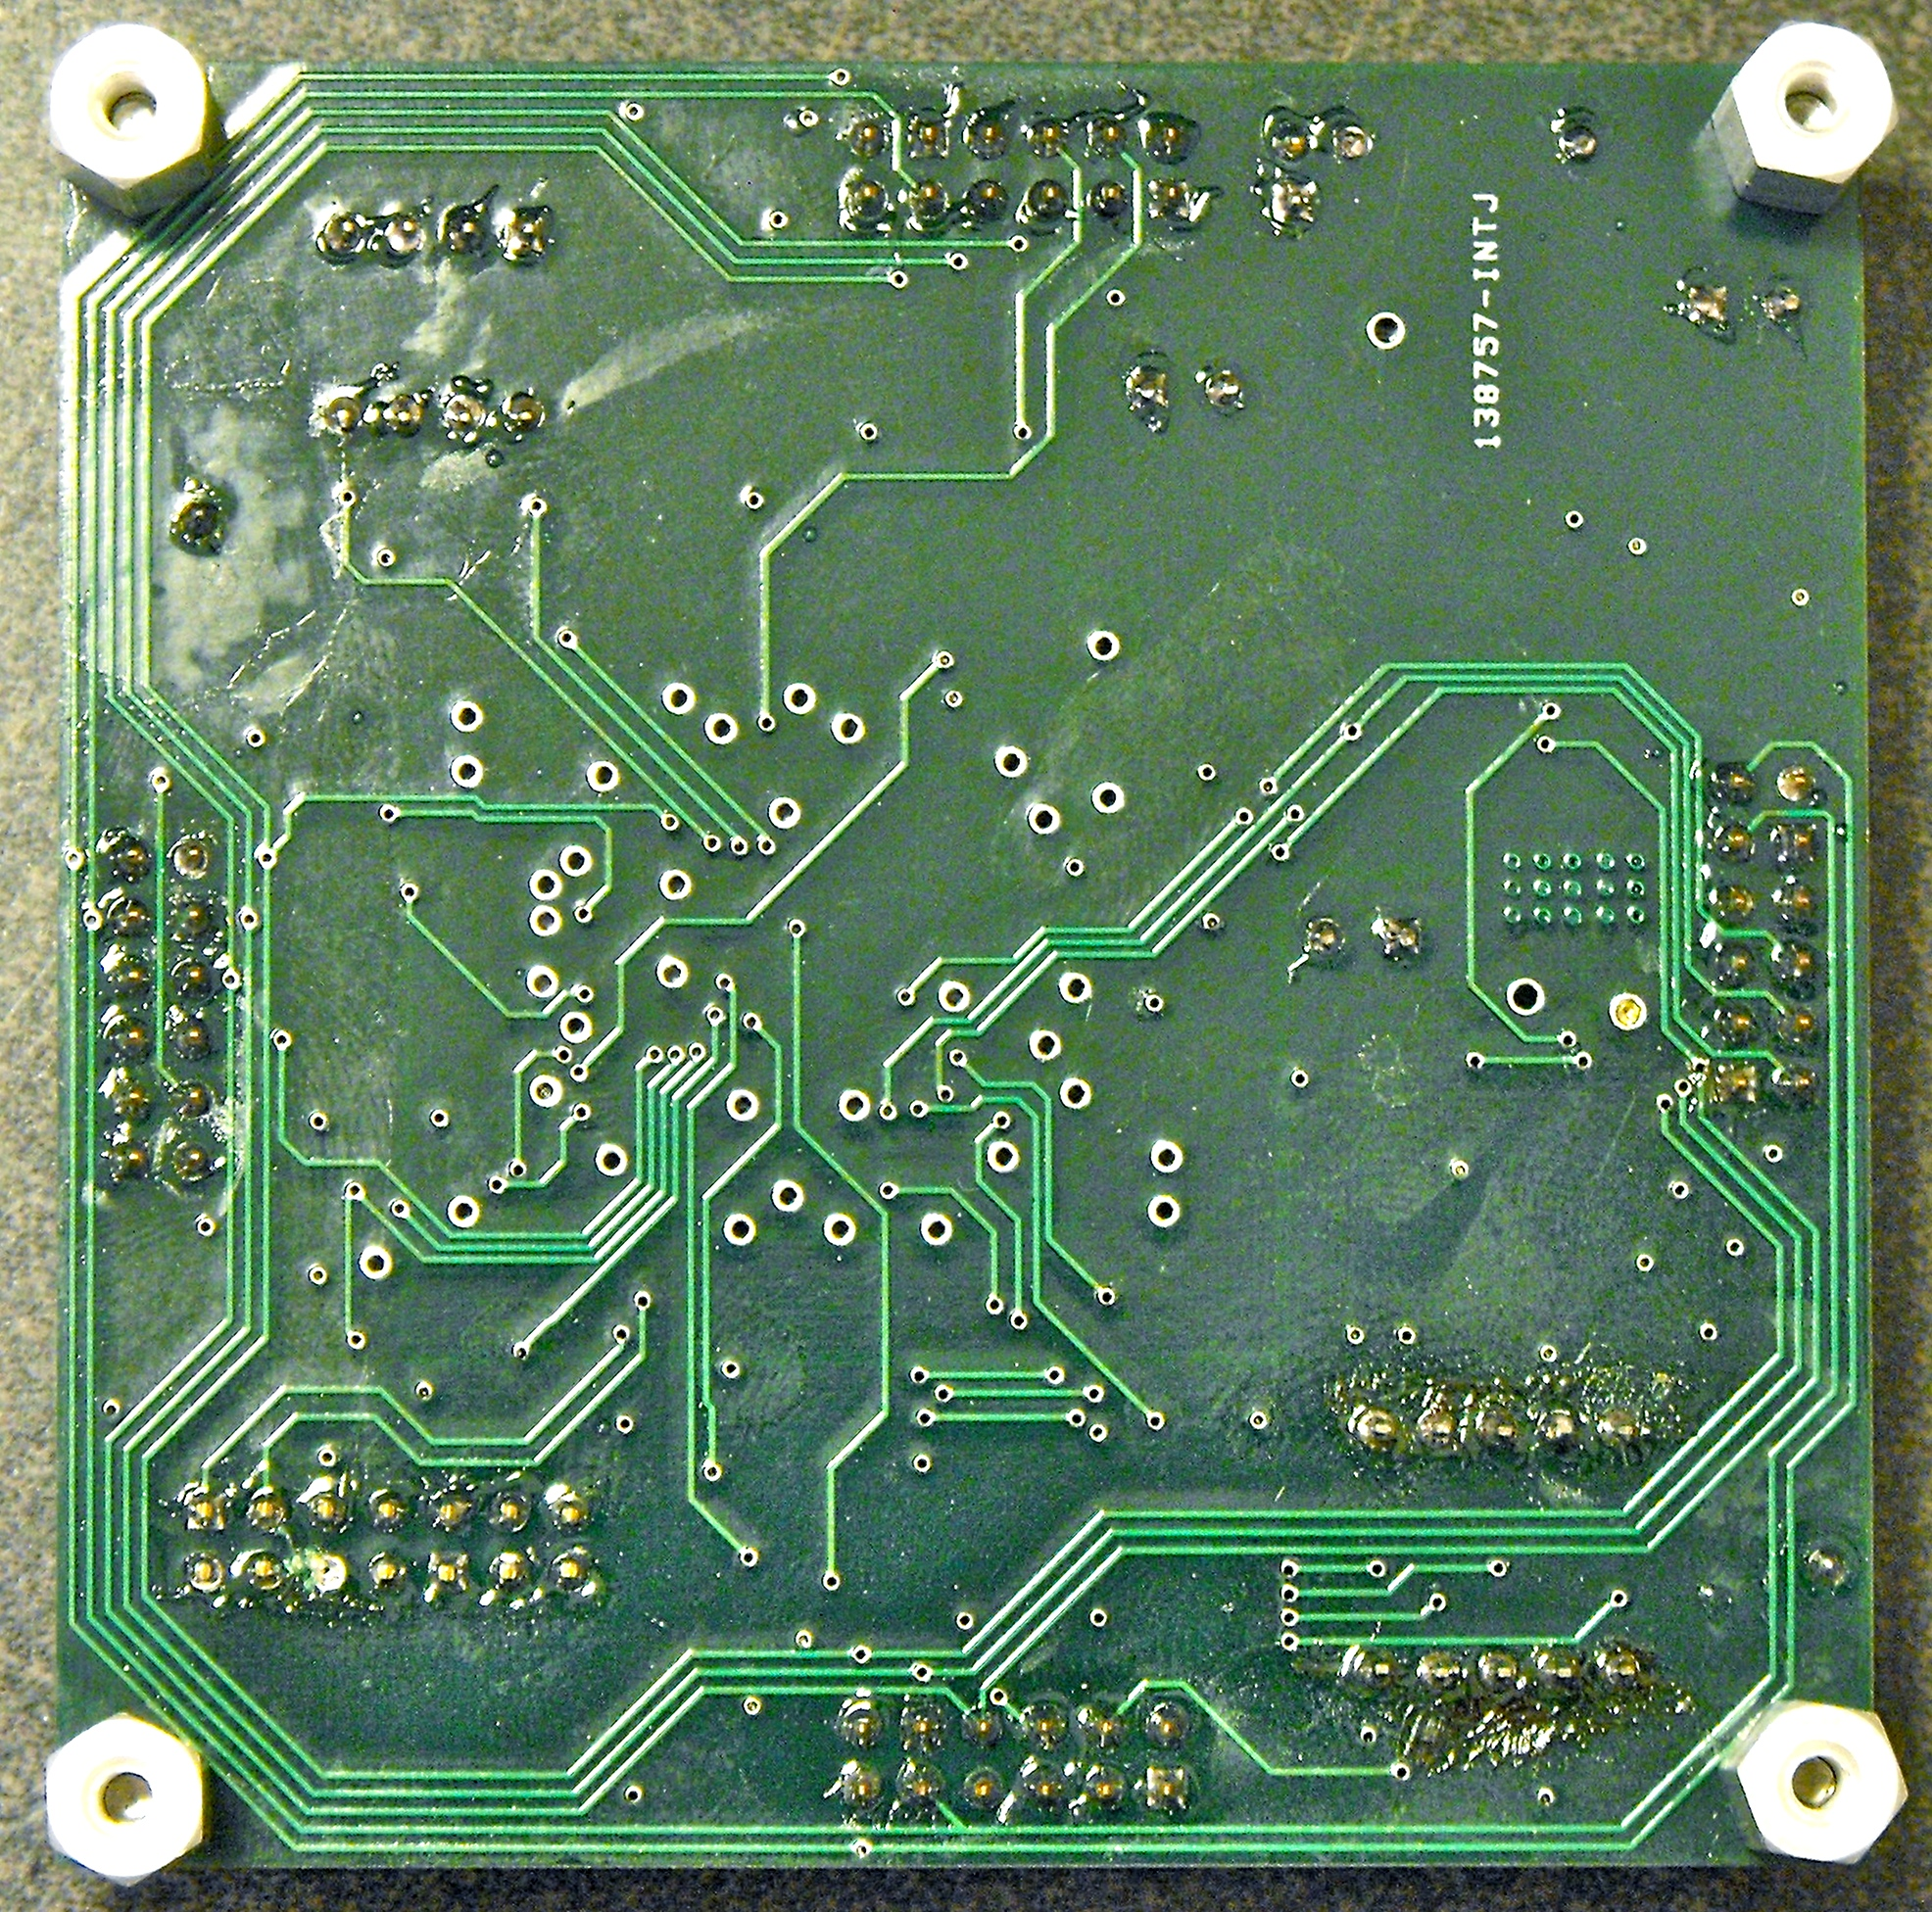
\includegraphics[width=6in]{Appendices/Figures/appendices-board_bottom.JPG}
		\caption{Bottom of the board}
		\label{fig:appendices:board_bottom}
	\end{centering}
\end{figure}

\chapter{Dynamic Memory Implementation}\label{sec:appendix:dynamic_memory}

Data transfers at the network and API level require the use of dynamic memory because messages can be of varying length. Texas Instruments provides a dynamic memory manager, but the version available for the project appeared to be dysfunctional. As an alternative, a custom memory manager was written that is described in this section. 

The memory manager has a dedicated memory pool from which it allocates. The memory manager monitors allocations through a look-up table. The look-up table stores the base address and memory length of each allocation. Both allocation and de-allocation are supported. When an allocation is requested, the memory manager uses the lowest available memory address with enough free space, including in between previous allocations. This helps to combat fragmentation, but if there are enough allocations, fragmentation would become an issue. Fortunately, there are very few allocations in the toolkit, so fragmentation is not an issue.

\chapter{Follow-up Monitor}\label{sec:appendix:follow_up_monitor}

Several parts of the toolkit require a follow-up action be executed at a later time, such as finding neighbors, data timeouts, etc. All of these cases use the ``follow-up monitor.'' The follow-up monitor provides capabilities for code to register a follow-up item to be run at a later date. A follow-up item consists of a callback function, an optional callback function argument, the follow-up rate, and whether this is a one shot follow-up, or should be called regularly. The follow-up monitor uses a single period function that manages the elapsed time of the follow-up items. Whenever it's time to run a follow-up item, the follow-up monitor calls the callback function. Follow-up items are added and (optionally) removed at run-time.

\chapter{Test Code} \label{sec:appendix:mpi_test_code}

The following code is shared between all nodes. A compile-time directive is defined to differentiate between the root and router. If the value \lstinline$IS_ROUTER$ is defined, then the node is a non-root router. If the value \lstinline$IS_ROOT$ is defined, then the node is the root. Both values cannot be defined at the same time. The test to run is defined by defining one of the compile-time directives \lstinline$TEST_SPI$, \lstinline$TEST_PROTOCOL$, or \lstinline$TEST_MPI$, which tests the physical/data link layer, network layer, and API respectively. Only one test can be defined at a time.

\begin{landscape}
\lstset{tabsize=2}
\lstinputlisting{Appendices/Service_TestService.c}
\end{landscape}

\chapter{Expanded Convolution Results}\label{sec:appendix:mpi_results}

\begin{figure}[ptb]
	\begin{centering}
		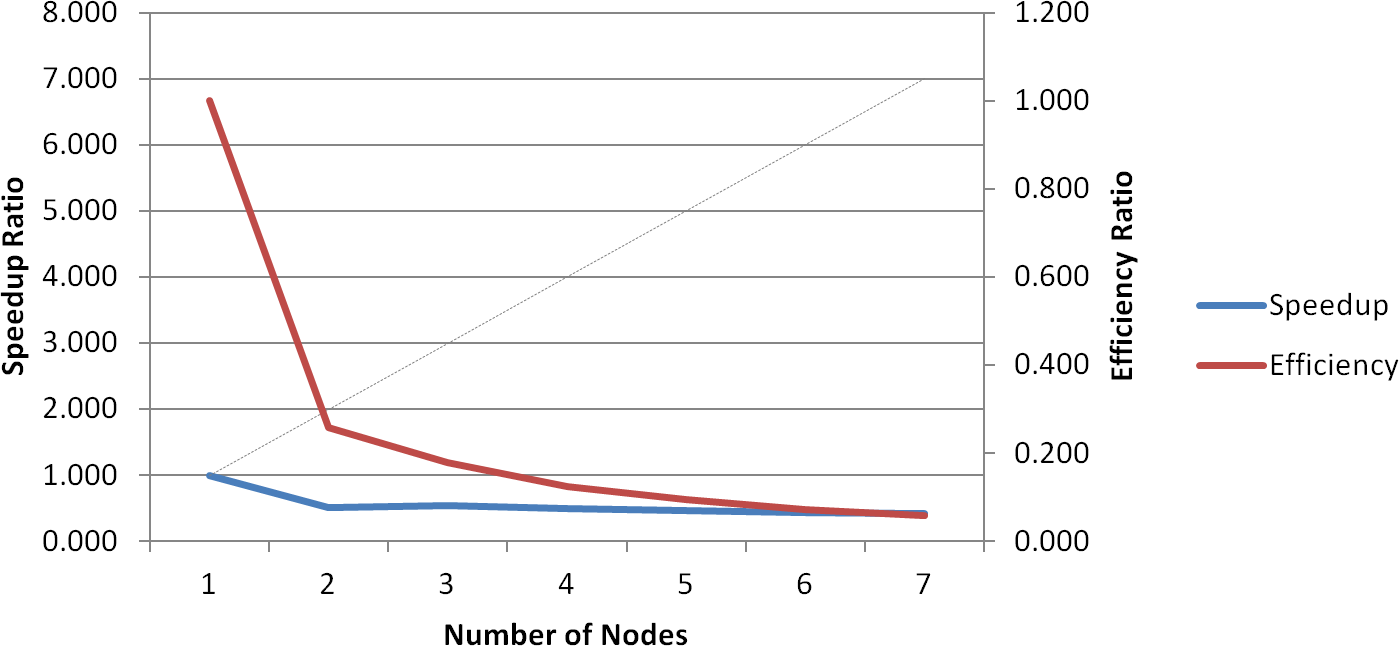
\includegraphics[width=6in]{Appendices/Figures/appendices-convolution_results_100.png}
		\caption{Speedup and efficiency versus number of nodes (100 byte data payload)}
		\label{fig:appendices:convolution_results_100}
	\end{centering}
\end{figure}

\begin{figure}[ptb]
	\begin{centering}
		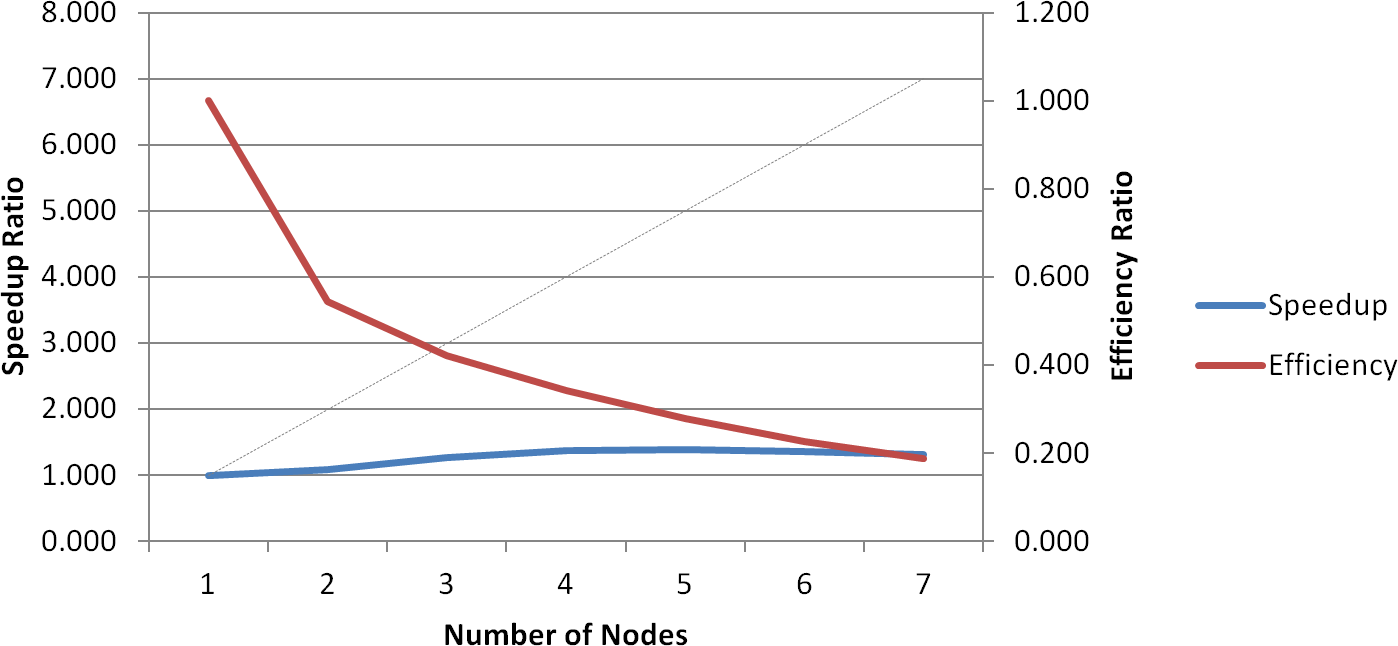
\includegraphics[width=6in]{Appendices/Figures/appendices-convolution_results_200.png}
		\caption{Speedup and efficiency versus number of nodes (200 byte data payload)}
		\label{fig:appendices:convolution_results_200}
	\end{centering}
\end{figure}

\begin{figure}[ptb]
	\begin{centering}
		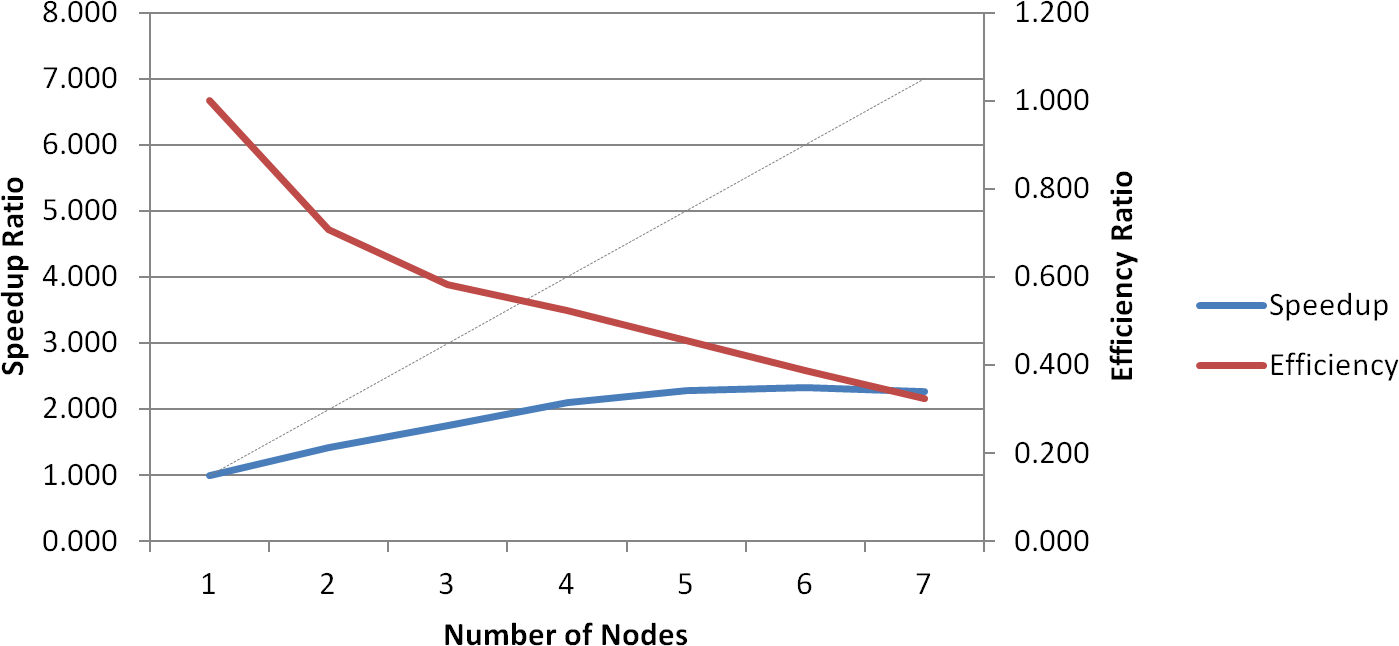
\includegraphics[width=6in]{Appendices/Figures/appendices-convolution_results_300.png}
		\caption{Speedup and efficiency versus number of nodes (300 byte data payload)}
		\label{fig:appendices:convolution_results_300}
	\end{centering}
\end{figure}

\begin{figure}[ptb]
	\begin{centering}
		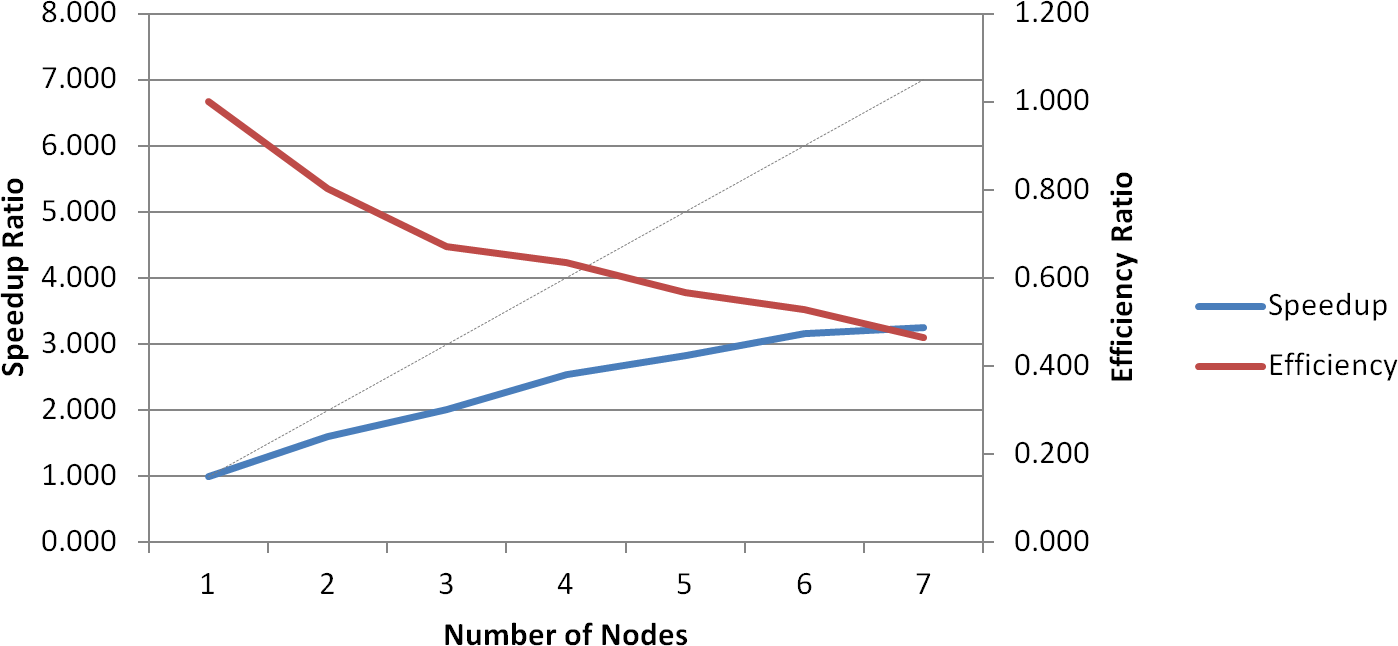
\includegraphics[width=6in]{Appendices/Figures/appendices-convolution_results_400.png}
		\caption{Speedup and efficiency versus number of nodes (400 byte data payload)}
		\label{fig:appendices:convolution_results_400}
	\end{centering}
\end{figure}

\begin{figure}[ptb]
	\begin{centering}
		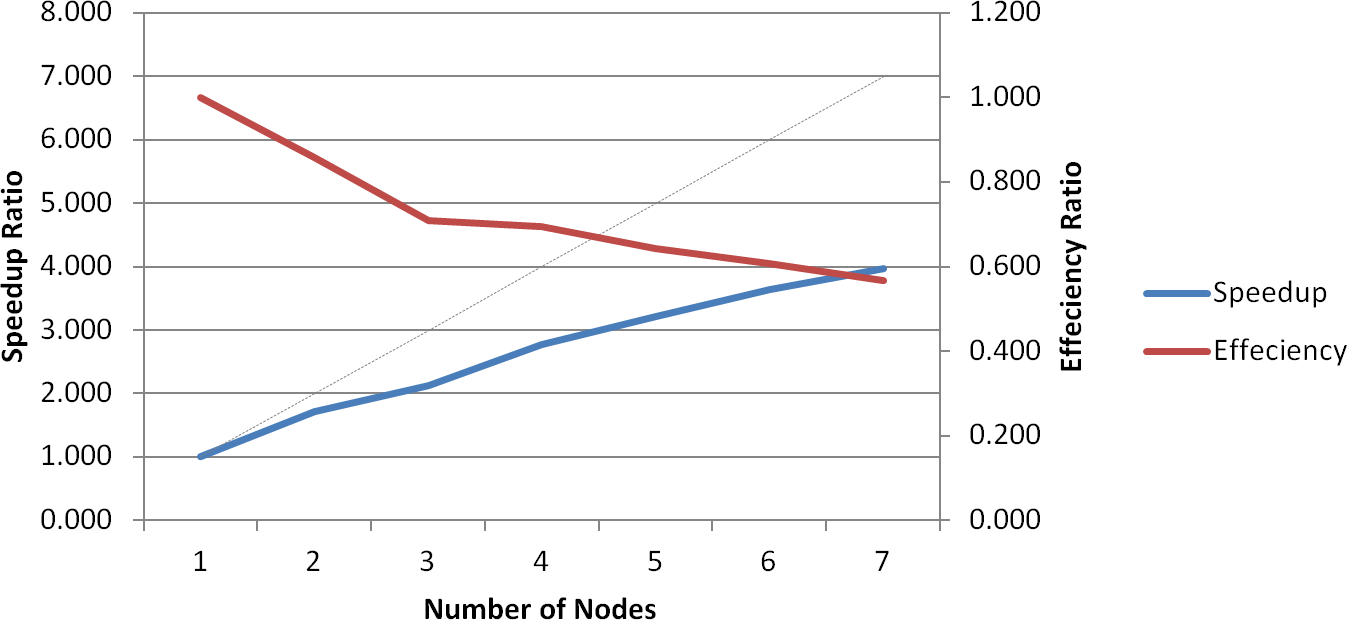
\includegraphics[width=6in]{Appendices/Figures/appendices-convolution_results_500.png}
		\caption{Speedup and efficiency versus number of nodes (500 byte data payload)}
		\label{fig:appendices:convolution_results_500}
	\end{centering}
\end{figure}

\begin{figure}[ptb]
	\begin{centering}
		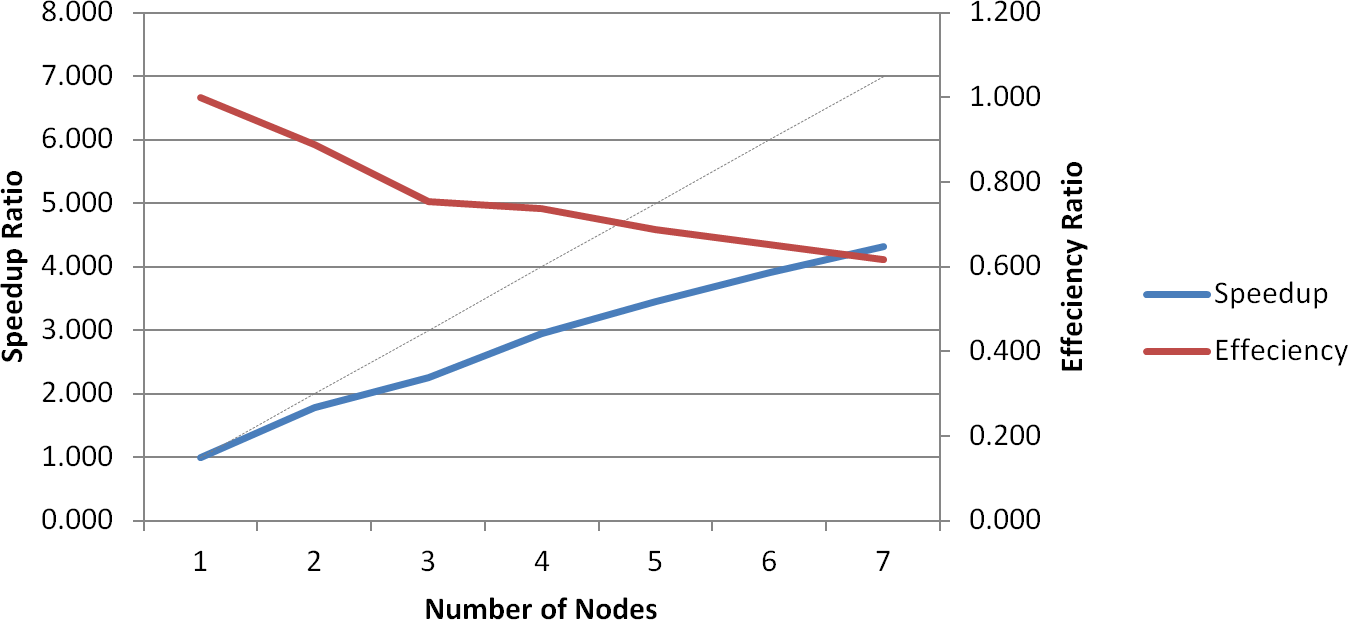
\includegraphics[width=6in]{Appendices/Figures/appendices-convolution_results_600.png}
		\caption{Speedup and efficiency versus number of nodes (600 byte data payload)}
		\label{fig:appendices:convolution_results_600}
	\end{centering}
\end{figure}

\begin{figure}[ptb]
	\begin{centering}
		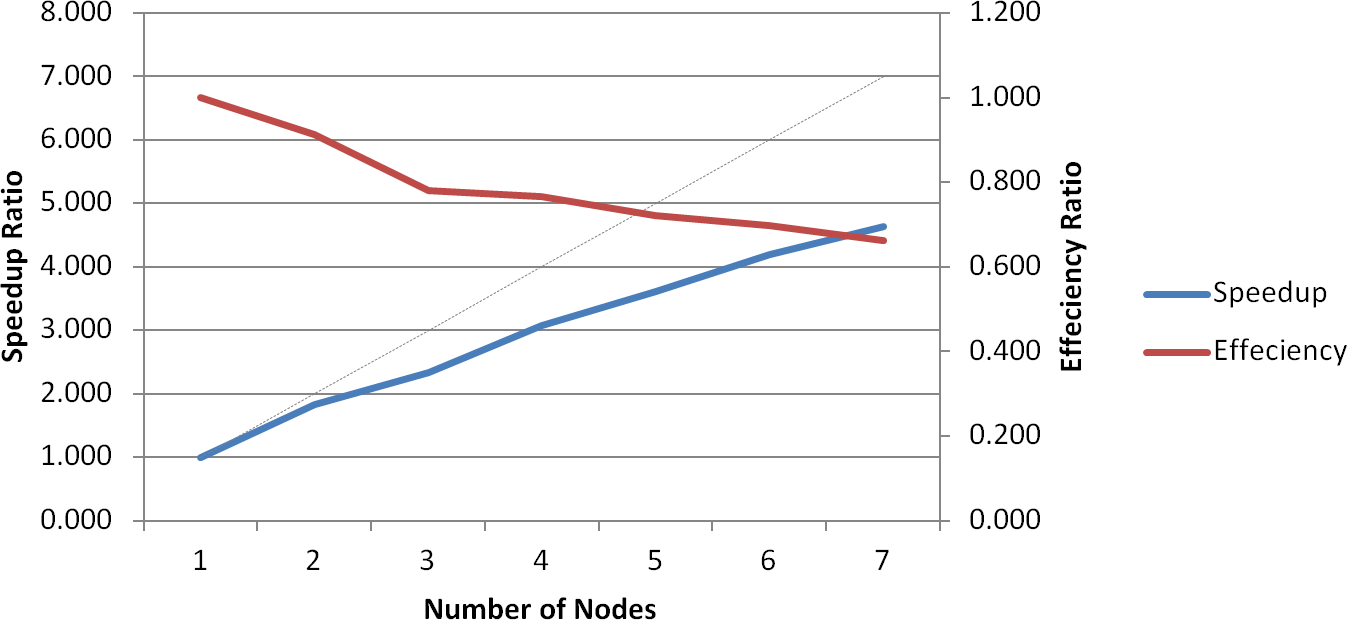
\includegraphics[width=6in]{Appendices/Figures/appendices-convolution_results_700.png}
		\caption{Speedup and efficiency versus number of nodes (700 byte data payload)}
		\label{fig:appendices:convolution_results_700}
	\end{centering}
\end{figure}

\end{appendices}

\chapter*{About the Author}

Bryan Hughes was born on September 27th, 1982 in Houston, TX and is the son of Russell and Suzanne Hughes and older sibling of Beth Hughes. The author lived briefly in Houston, TX and Truth or Consequences, NM before moving to Denton, TX, where he lived during most of his years in grade school. After graduating from Billy Ryan High School in 2001, he began studying electrical engineering and computer science at Texas Tech University. In the spring of 2005, Bryan accepted an internship at Walt Disney World Resort in Orlando, FL, where he developed control systems for water features at the theme parks. The author received his Bachelor of Science degree in Electrical Engineering, with a minor in Computer Science, in the summer of 2006. He married Melissa Hughes in December of 2006, who received her Master of Science degree in Food Science in 2009. Bryan began pursuing his doctorate immediately after receiving his bachelor's degree under the supervision of Dr. Brian Nutter, becoming the first person in 20 years to skip his master's degree in the department. During his graduate studies, he was a teaching assistant and instructor of a laboratory class for three years. Bryan was also a research assistant for one year, where he helped develop a new image compression method. The author also became the lab manager and IT administrator for the Computer Vision and Image Analysis Laboratory. In 2009, he qualified for a non-thesis Master of Science degree in Electrical Engineering during the course of his doctoral studies. Bryan is an active member of the Association for Computing Machinery (ACM) and the Institute for Electrical and Electronics Engineers (IEEE), and he has several conference and journal publications.